
\documentclass[12pt]{article}

\usepackage{amsmath, amssymb, amsthm}
\usepackage{enumitem}
\usepackage{hyperref}
\usepackage{geometry}
\usepackage{graphicx}
\geometry{a4paper, margin=1in}

% Define theorem styles
\newtheorem{theorem}{Theorem}
\newtheorem{lemma}[theorem]{Lemma}
\newtheorem{proposition}[theorem]{Proposition}
\newtheorem{corollary}[theorem]{Corollary}
\newtheorem{definition}[theorem]{Definition}
\renewcommand{\qedsymbol}{$\blacksquare$} % Use a black square for QED

% Document title and author
\title{Tree equivalence theorem contains a mistake}
\author{Heorhii Lopattn}
\date{\today}

\begin{document}
\newcommand{\fire}[1]{\xrightarrow{#1}}
\newcommand{\firee}[1]{\,[#1\rangle} % For enabled and fires, if needed
\newcommand{\marking}[1]{\mathbf{#1}} % For marking notation like [in] or [o]
\newcommand{\placeset}{\mathcal{P}}
\newcommand{\transitionset}{\mathcal{T}}
\newcommand{\flowrel}{\mathcal{F}}
\newcommand{\reachable}[2]{\mathcal{R}(#1, #2)}


\maketitle



\section*{Solution}
A theorem presented in Piotr Chrząstowski-Wachtel, Boualem Benatallah, Rachid Hamadi, Milton O'Dell, Adi Susanto, Top-down Petri Net Based Approach to Dynamic Workflow Modelling, 2003 states the following:

% no blank lines before this
\begin{center}
  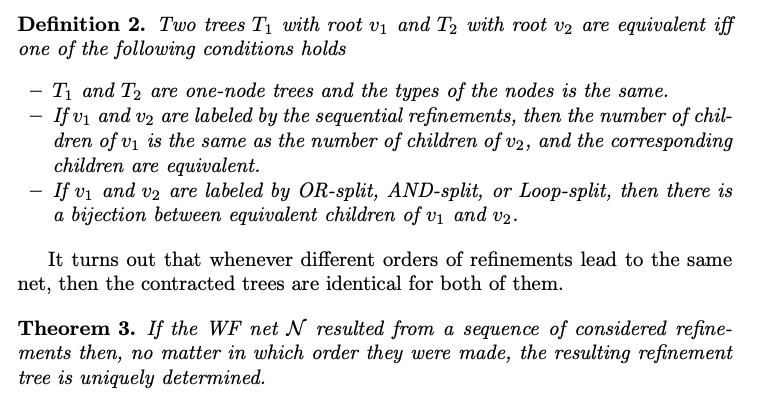
\includegraphics[
    width=\textwidth,        % full text width
    height=0.8\textheight,   % but no taller than 80% of text height
    keepaspectratio          % preserve aspect ratio
  ]{theorem.png}
  \label{fig:theorem}
\end{center}
\newpage
The theorem contains a mistake. Observe that a sequence: Loop from place $v$; Loop from place $v$ \\
Is the same as: Loop from a place $v$, "or" transformation from the loop transition.
The trees are obviously can't be equivalent according to the equivalence definition, which contradicts the theorem. \\
To fix the theorem, during the "compression" of a tree we can force the following changes: \\
When a node $o$ of type "or" is a children of a node $l$ of type "loop", we bring all children of $o$ to be children of $l$, then remove $o$. \\
Since  no other sequence of transformations is equivalent to some different one, this fixes the theorem.
\end{document}
